\newpage


\section{Actividad 5: Polarización y func. del TRIAC}


\subsection{Actividad de Laboratorio}

\begin{itemize}
    \item TRIAC BT137
    \item DIAC DB3
    \item Dos Multimetros
    \item Dos fuentes de alimentación
    \item Potenciómetro $5k\Omega$
\end{itemize}

\paragraph{Procedimiento}
Para esta actividad se implementó el siguiente circuito:\\
\includegraphics[width=8cm]{./imagenes/Circ5.png}

Primero variamos el potenciómetro de forma que $V_G$ quede a potencial de cero volts cuando la fuente esta conectada.\\
Ahora colocamos la fuente de alimentación en 50V y aumentamos lentamente $V_G$ observando permanentemente $I_G$ e $I_A$. Determinamos el momento donde el dispositivo se dispara.\\
Bajamos el valor de $V_G$ a cero y observamos lo que pasa con $I_A$.\\
Ahora subimos El valor de Vcc a 100V y repetimos los pasos anteriores. \\
Luego subimos El valor de Vcc a 150V y repetimos los pasos anteriores.\\
Y finalmente obtenemos el siguiente grafico dado por las siguientes tablas:

\begin{figure}[ht]
\centering
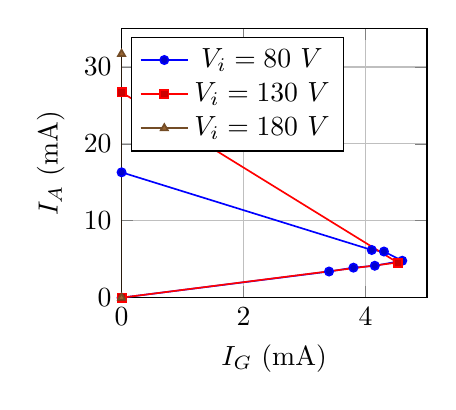
\begin{tikzpicture}
\begin{axis}[
    width=0.45\textwidth,
    height=5cm,
    xlabel={$I_G$ (mA)},
    ylabel={$I_A$ (mA)},
    xmin=0, xmax=5,
    ymin=0, ymax=35,
    legend pos=north west,
    grid=both,
    semithick,
    mark size=1.5pt
]
\addplot+[mark=*] coordinates {
(0,0) (3.4,3.4) (3.8,3.9) (4.15,4.15) (4.6,4.8) (4.3,6) (4.1,6.2) (0,16.3)
};
\addlegendentry{$V_i=80\ \text{V}$}

\addplot+[mark=square*] coordinates {
(0,0) (4.53,4.57) (4.53,4.53) (0,26.7)
};
\addlegendentry{$V_i=130\ \text{V}$}

\addplot+[mark=triangle*] coordinates {
(0,0) (0,31.7)
};
\addlegendentry{$V_i=180\ \text{V}$}

\end{axis}
\end{tikzpicture}
\caption{Curvas $I_A$ vs $I_G$ para las tres tensiones de alimentación.}
\label{fig:IA_vs_IG}
\end{figure}


\begin{table}[ht]
\centering
\setlength{\tabcolsep}{3pt} % reducir separacion de columnas
\renewcommand{\arraystretch}{0.9}% reducir alto de filas
\begin{minipage}[t]{0.48\textwidth}
\centering
\small
\begin{tabular}{|ccc|ccc|}
\hline
\rowcolor[HTML]{FFCE93} 
\multicolumn{3}{|c|}{\cellcolor[HTML]{FFCE93}$V_i$=80V}       & \multicolumn{3}{c|}{\cellcolor[HTML]{FFCE93}$V_i$=130V}      \\ \hline
\rowcolor[HTML]{9AFF99} 
\multicolumn{1}{|c|}{\cellcolor[HTML]{9AFF99}$V_G${[}V{]}} &
  \multicolumn{1}{c|}{\cellcolor[HTML]{9AFF99}$I_G${[}mA{]}} &
  $I_A${[}mA{]} &
  \multicolumn{1}{c|}{\cellcolor[HTML]{9AFF99}$V_G${[}V{]}} &
  \multicolumn{1}{c|}{\cellcolor[HTML]{9AFF99}$I_G${[}mA{]}} &
  $I_A${[}mA{]} \\ \hline
\multicolumn{1}{|c|}{0}    & \multicolumn{1}{c|}{0}    & 0    & \multicolumn{1}{c|}{0}    & \multicolumn{1}{c|}{0}    & 0    \\ \hline
\multicolumn{1}{|c|}{10}   & \multicolumn{1}{c|}{0}    & 0    & \multicolumn{1}{c|}{10}   & \multicolumn{1}{c|}{0}    & 0    \\ \hline
\multicolumn{1}{|c|}{20}   & \multicolumn{1}{c|}{0}    & 0    & \multicolumn{1}{c|}{20}   & \multicolumn{1}{c|}{0}    & 0    \\ \hline
\multicolumn{1}{|c|}{30}   & \multicolumn{1}{c|}{0}    & 0    & \multicolumn{1}{c|}{30}   & \multicolumn{1}{c|}{0}    & 0    \\ \hline
\multicolumn{1}{|c|}{31}   & \multicolumn{1}{c|}{0}    & 0    & \multicolumn{1}{c|}{31}   & \multicolumn{1}{c|}{0}    & 0    \\ \hline
\multicolumn{1}{|c|}{32}   & \multicolumn{1}{c|}{3.4}  & 3.4  & \multicolumn{1}{c|}{31.6} & \multicolumn{1}{c|}{4.53} & 4.57 \\ \hline
\multicolumn{1}{|c|}{23.3} & \multicolumn{1}{c|}{3.8}  & 3.9  & \multicolumn{1}{c|}{28.4} & \multicolumn{1}{c|}{4.53} & 4.53 \\ \hline
\multicolumn{1}{|c|}{23.1} & \multicolumn{1}{c|}{4.15} & 4.15 & \multicolumn{1}{c|}{0.3}  & \multicolumn{1}{c|}{0}    & 26.7 \\ \hline
\multicolumn{1}{|c|}{23.2} & \multicolumn{1}{c|}{4.6}  & 4.8  & \multicolumn{1}{c|}{-}    & \multicolumn{1}{c|}{-}    & -    \\ \hline
\multicolumn{1}{|c|}{23.2} & \multicolumn{1}{c|}{4.3}  & 6    & \multicolumn{1}{c|}{-}    & \multicolumn{1}{c|}{-}    & -    \\ \hline
\multicolumn{1}{|c|}{23.3} & \multicolumn{1}{c|}{4.1}  & 6.2  & \multicolumn{1}{c|}{-}    & \multicolumn{1}{c|}{-}    & -    \\ \hline
\multicolumn{1}{|c|}{0.7}  & \multicolumn{1}{c|}{0}    & 16.3 & \multicolumn{1}{c|}{-}    & \multicolumn{1}{c|}{-}    & -    \\ \hline
\end{tabular}
\end{minipage}
\begin{minipage}[t]{0.32\textwidth}
\centering
\small
\begin{tabular}{|ccc|}
\hline
\rowcolor[HTML]{FFCE93} 
\multicolumn{3}{|c|}{\cellcolor[HTML]{FFCE93}$V_i$=180V} \\ \hline
\rowcolor[HTML]{9AFF99} 
\multicolumn{1}{|c|}{\cellcolor[HTML]{9AFF99}$V_G${[}V{]}} & \multicolumn{1}{c|}{\cellcolor[HTML]{9AFF99}$I_G${[}mA{]}} & $I_A${[}mA{]} \\ \hline
\multicolumn{1}{|c|}{0}  & \multicolumn{1}{c|}{0} & 0    \\ \hline
\multicolumn{1}{|c|}{10} & \multicolumn{1}{c|}{0} & 0    \\ \hline
\multicolumn{1}{|c|}{20} & \multicolumn{1}{c|}{0} & 0    \\ \hline
\multicolumn{1}{|c|}{30} & \multicolumn{1}{c|}{0} & 0    \\ \hline
\multicolumn{1}{|c|}{32} & \multicolumn{1}{c|}{0} & 31.7 \\ \hline
\multicolumn{1}{|c|}{-}  & \multicolumn{1}{c|}{-} & -    \\ \hline
\multicolumn{1}{|c|}{-}  & \multicolumn{1}{c|}{-} & -    \\ \hline
\multicolumn{1}{|c|}{-}  & \multicolumn{1}{c|}{-} & -    \\ \hline
\multicolumn{1}{|c|}{-}  & \multicolumn{1}{c|}{-} & -    \\ \hline
\multicolumn{1}{|c|}{-}  & \multicolumn{1}{c|}{-} & -    \\ \hline
\multicolumn{1}{|c|}{-}  & \multicolumn{1}{c|}{-} & -    \\ \hline
\end{tabular}
\end{minipage}
\end{table}

\paragraph{Análisis de Resultados}

Según las tablas obtenidas podemos ver como para mayores valores de tensión de alimentación, el TRIAC se dispara con menores valores de corriente de compuerta. Esto se debe a que al aumentar la tensión de alimentación, la corriente a través del dispositivo también aumenta, lo que facilita el disparo del TRIAC con una corriente de compuerta menor.\\
Con respecto al grafico comparando $I_A$ vs $I_G$, podemos observar que efectivamente cuando se aumenta la tensión de alimentación, se necesitan menores valores de corriente de compuerta para que el TRIAC conduzca. Lo unico malo fue que para 180V el disparo ocurre tan rápido que no pudimos medir la corriente de compuerta, pero si la corriente de anodo.\\
